\documentclass[12pt, a4paper]{article}

% Pacotes para fontes e codificação
\usepackage[utf8]{inputenc}
\usepackage[T1]{fontenc}
\usepackage[brazil]{babel}

% Pacote para fonte Arial (ou similar sem serifa)
\usepackage{helvet}
\renewcommand{\familydefault}{\sfdefault} % Configura a fonte sem serifa como padrão

% Configuração das margens
\usepackage[margin=2.5cm]{geometry}

% Pacotes para imagens, tabelas e afins
\usepackage{graphicx}
\usepackage{float}
\usepackage{booktabs}
\usepackage{amsmath}
\usepackage{hyperref}

\begin{document}

\title{\textbf{Avaliação Empírica de Algoritmos para o Problema da Mochila 0-1 com Duas Restrições}}
\author{Arthur Teixeira, Daniel Bigonha, Rafael Stylita e Arthur Junqueira}
\date{} % Sem data

\maketitle

\begin{abstract}
O Problema da Mochila 0-1 (Knapsack Problem) é um clássico problema de otimização combinatória. Este trabalho investiga uma variante deste problema, incorporando uma segunda restrição (volume, além do peso), para a qual foram implementadas três diferentes abordagens algorítmicas: Backtracking, Branch and Bound e Programação Dinâmica. O objetivo central é realizar uma avaliação empírica do desempenho (tempo de execução e nós visitados) de cada estratégia à medida que as dimensões do problema crescem. Os resultados experimentais, baseados em mais de 10.000 instâncias de teste e avaliados por testes estatísticos (Friedman), confirmam a superioridade da Programação Dinâmica para restrições pequenas a moderadas e evidenciam a eficácia do algoritmo Branch and Bound sobre o Backtracking na poda do espaço de busca.
\end{abstract}

\section{Introdução}
O Problema da Mochila 0-1 (Knapsack Problem) é um dos problemas mais estudados na ciência da computação e pesquisa operacional. A versão clássica consiste em selecionar um subconjunto de itens, cada um com um peso e um valor associados, de modo a maximizar o valor total sem exceder a capacidade de peso da mochila. Neste trabalho, abordamos uma variação bidimensional deste problema, onde há duas restrições simultâneas: um peso máximo $W$ e um volume máximo $V$. Cada item disponível $i$ possui um valor $v_i$, um peso $w_i$ e um volume $l_i$.

O objetivo principal deste trabalho prático é projetar, implementar e realizar uma análise empírica rigorosa de três algoritmos exatos para solucionar essa variação da mochila: Programação Dinâmica, Backtracking e Branch and Bound. 

Resumidamente, os resultados obtidos comprovam as análises teóricas de complexidade esperadas. Demonstrou-se estatisticamente que a Programação Dinâmica oferece o menor tempo de execução para instâncias onde $W$ e $V$ são relativamente pequenos. Entretanto, sua natureza pseudo-polinomial a torna inviável para grandes capacidades. Em contrapartida, o método Branch and Bound mostrou-se imune ao tamanho das capacidades e muito superior ao Backtracking puro devido ao uso eficiente de limitantes superiores que podam substancialmente a árvore de busca recursiva.

O restante deste trabalho está organizado da seguinte forma: a Seção 2 detalha os algoritmos implementados e suas complexidades teóricas. A Seção 3 apresenta a metodologia da avaliação experimental e discute os resultados obtidos através de gráficos e testes estatísticos. A Seção 4 apresenta a conclusão do estudo. As referências bibliográficas encerram o documento.

\section{Descrição dos Algoritmos e Complexidades}

\subsection{Programação Dinâmica}
A Programação Dinâmica resolve o problema resolvendo subproblemas menores e armazenando seus resultados para evitar recálculos. Para a mochila bidimensional, utilizamos uma matriz tridimensional implícita onde os eixos são os itens, a capacidade de peso e a capacidade de volume. Para economizar espaço, a implementação foi otimizada para manter apenas o estado atual, armazenando as decisões em uma estrutura auxiliar mais leve (bits/booleanos) para posterior reconstrução da solução ótima.
\begin{itemize}
    \item \textbf{Complexidade de Tempo:} $\mathcal{O}(N \cdot W \cdot V)$, onde $N$ é o número de itens, $W$ é o peso máximo e $V$ o volume máximo. Esta complexidade é dita pseudo-polinomial.
    \item \textbf{Complexidade de Espaço:} $\mathcal{O}(W \cdot V)$ para o cálculo do valor máximo, mais a estrutura de decisões $\mathcal{O}(N \cdot W \cdot V)$ para a reconstrução dos itens selecionados.
\end{itemize}

\subsection{Backtracking}
O Backtracking realiza uma busca exaustiva estruturada no espaço de soluções (representado como uma árvore binária onde escolhe-se incluir ou não um item). Ele tenta todas as combinações possíveis e retrocede (faz *backtrack*) apenas quando o peso ou o volume do item ultrapassam a capacidade restante da mochila. Nenhuma heurística avançada é utilizada para prever se um caminho levará a um lucro subótimo.
\begin{itemize}
    \item \textbf{Complexidade de Tempo:} $\mathcal{O}(2^N)$ no pior caso. O algoritmo explora todas as folhas viáveis da árvore.
    \item \textbf{Complexidade de Espaço:} $\mathcal{O}(N)$, que é a altura máxima da pilha de chamadas recursivas.
\end{itemize}

\subsection{Branch and Bound}
O algoritmo Branch and Bound melhora o Backtracking incorporando a técnica de poda (*pruning*). Em cada nó da árvore de decisão, calcula-se um limitante superior (relaxação fracionária do problema) para o melhor lucro possível caso continuemos a explorar aquele ramo. Se esse limitante for menor ou igual à melhor solução inteira já encontrada, o ramo inteiro é descartado. 
\begin{itemize}
    \item \textbf{Complexidade de Tempo:} $\mathcal{O}(2^N)$ no pior caso teórico. No entanto, o tempo prático é significativamente menor do que o Backtracking devido ao corte de grande parte da árvore de busca.
    \item \textbf{Complexidade de Espaço:} $\mathcal{O}(N)$, semelhante ao Backtracking, pois a busca é feita em profundidade (DFS) mantendo o estado da recursão.
\end{itemize}

\section{Avaliação Experimental}

\subsection{Configuração dos Experimentos e Métricas}
Os experimentos foram configurados variando-se três parâmetros independentes: a quantidade de itens ($N$), o peso máximo suportado ($W$) e o volume máximo suportado ($V$). O ambiente de teste estipulou 10 instâncias geradas pseudo-aleatoriamente para cada combinação única de $(N, W, V)$. O tempo limite estabelecido por execução foi de 2.0 segundos.

As métricas de avaliação extraídas foram o \textbf{Tempo de Execução} (em segundos) e a \textbf{Quantidade de Nós Visitados} (para os métodos em árvore). Para validar a existência ou ausência de similaridade estatística de tempo entre os três métodos, aplicou-se o teste não-paramétrico de Friedman com nível de significância de 5\% (p-valor < $0.05$).

\subsection{Resultados e Comentários}

O Teste de Friedman indicou, na absoluta maioria dos cenários (com p-valores na ordem de $10^{-4}$ ou menores), que não houve empate estatístico entre as abordagens. Isso confirma que os desempenhos práticos são inerentemente distintos, o que corroboramos visualmente pelas análises de crescimento a seguir.

\subsubsection{Crescimento em Função de N, W e V}

A Figura \ref{fig:plot_n} exibe o comportamento isolado da escalabilidade em relação à quantidade de itens. Fica evidente a explosão combinatória $\mathcal{O}(2^N)$ do Backtracking puro, atingindo rapidamente a barreira do limite de tempo antes mesmo de $N=30$. A Programação Dinâmica, como esperado, varia de forma mais tênue nestas proporções de $N$.

\begin{figure}[H]
    \centering
    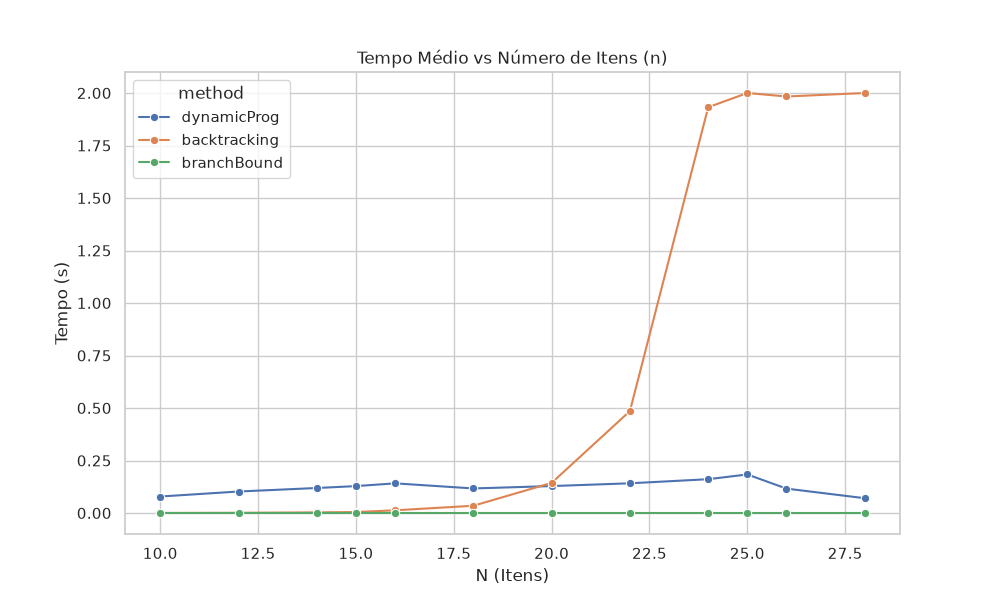
\includegraphics[width=0.7\textwidth]{scripts/plot_n.png}
    \caption{Tempo de execução vs Quantidade de itens (N)}
    \label{fig:plot_n}
\end{figure}

Por outro lado, quando avaliamos o crescimento das capacidades ($W$ e $V$), os algoritmos de busca (Backtracking e Branch and Bound) demonstram imunidade ao tamanho da mochila, pois suas complexidades baseiam-se apenas em $N$. Entretanto, como as Figuras \ref{fig:plot_w} e \ref{fig:plot_v} evidenciam claramente, a Programação Dinâmica sofre o impacto de sua complexidade espacial e temporal multiplicativa, tendo o seu tempo encarecido quase linearmente com a expansão de $W$ e $V$.

\begin{figure}[H]
    \centering
    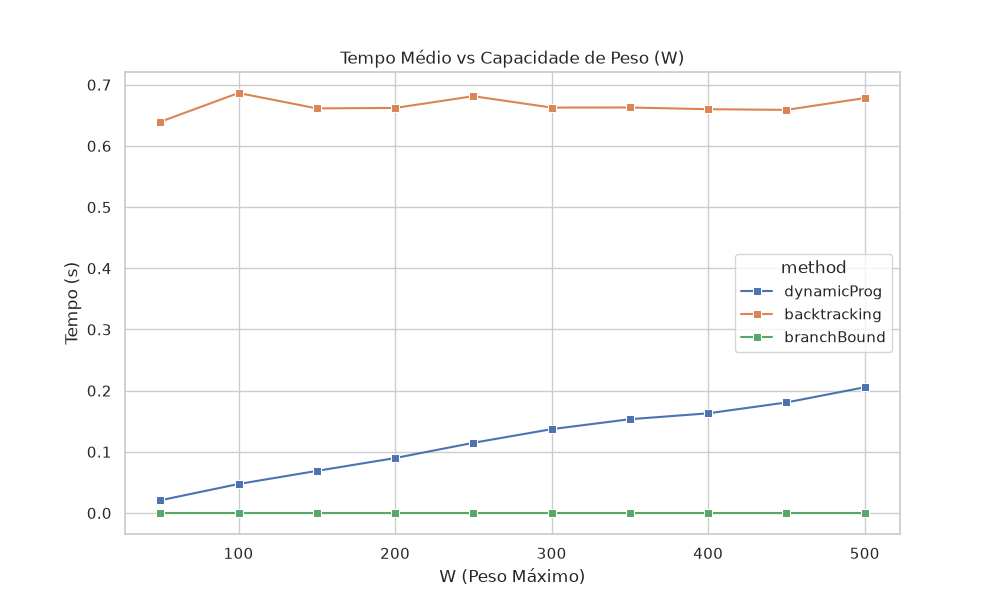
\includegraphics[width=0.7\textwidth]{scripts/plot_w.png}
    \caption{Tempo de execução vs Peso suportado (W)}
    \label{fig:plot_w}
\end{figure}

\begin{figure}[H]
    \centering
    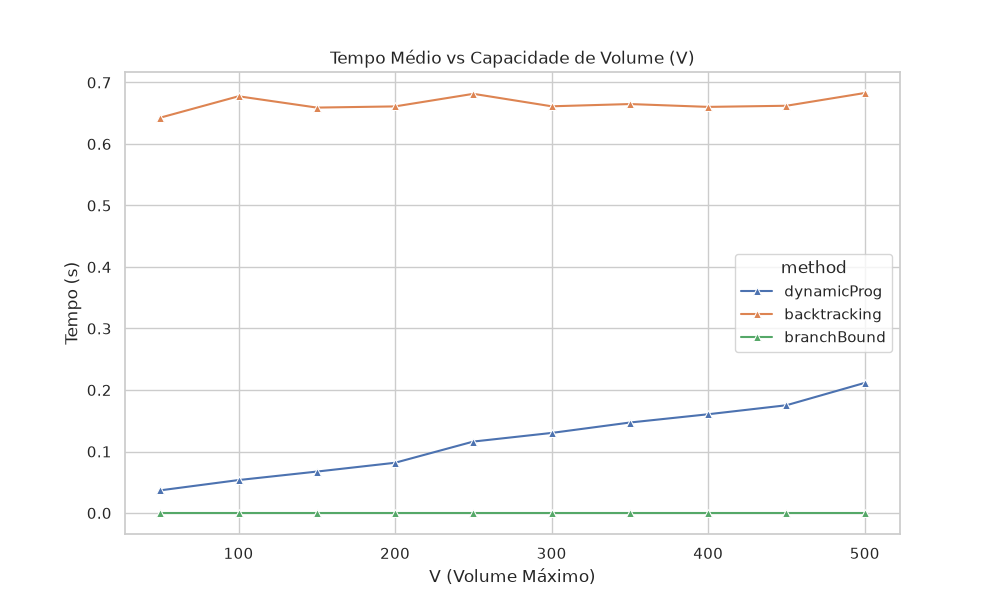
\includegraphics[width=0.7\textwidth]{scripts/plot_v.png}
    \caption{Tempo de execução vs Volume suportado (V)}
    \label{fig:plot_v}
\end{figure}

\subsubsection{Análise da Árvore de Busca e Poda}

Um dos resultados empíricos mais notáveis do projeto encontra-se na discrepância entre a quantidade de nós avaliados pelo Backtracking em oposição ao Branch and Bound (Figura \ref{fig:plot_nodes}). O gráfico foi construído em escala logarítmica para comportar a diferença estratosférica de eficiência. Enquanto a força bruta expande o espaço cego gerando dezenas de milhões de nós avaliados, a heurística de limite superior adotada pelo Branch and Bound extingue ramos inviáveis precocemente, conseguindo resultados em frações de milissegundos nas mesmas instâncias testadas.

\begin{figure}[H]
    \centering
    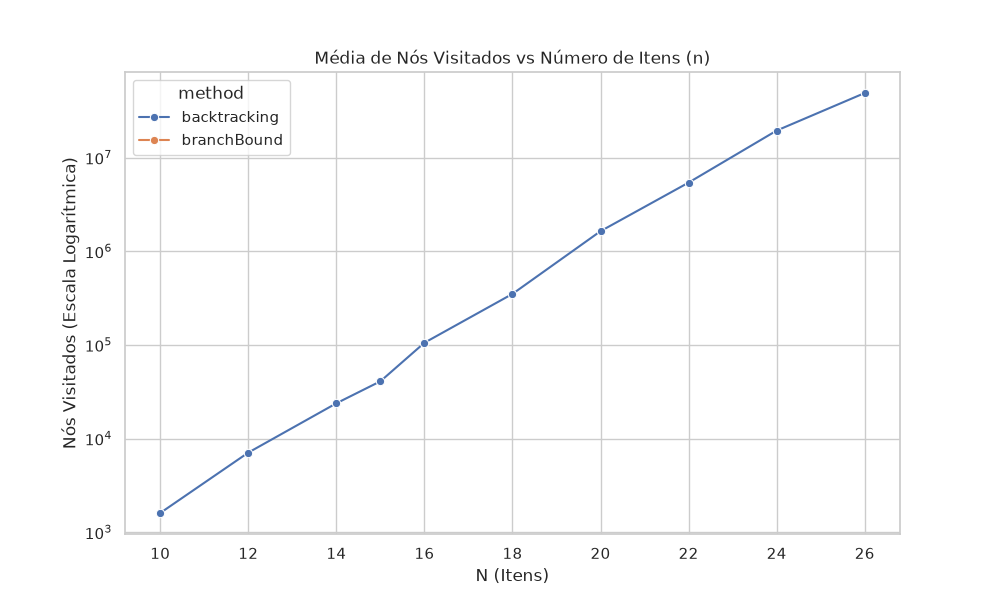
\includegraphics[width=0.7\textwidth]{scripts/plot_nodes.png}
    \caption{Nós visitados em escala logarítmica vs Quantidade de Itens (N)}
    \label{fig:plot_nodes}
\end{figure}

\section{Conclusão}
A experimentação prática realizada atendeu perfeitamente ao objetivo de expor os compromissos (trade-offs) inerentes ao design de algoritmos para o Problema da Mochila 0-1 bidimensional. Comprovamos que não existe uma "bala de prata". Para instâncias com limites operacionais (peso e volume) muito curtos ou moderados, a Programação Dinâmica mostrou-se soberana. Contudo, para cenários industriais onde os limites de carga e espaço sejam gigantescos, suas matrizes explodem a memória e o tempo alocados. 

Nesses casos, a abordagem por árvore se faz necessária, e demonstramos exaustivamente que a utilização de limitantes e relaxamento fracionário presente no Branch and Bound é estritamente vital, dado que o Backtracking primitivo sequer termina a execução para conjuntos ligeiramente maiores do que 25 itens.

\begin{thebibliography}{9}
\bibitem{cormen} 
Cormen, T. H., Leiserson, C. E., Rivest, R. L., e Stein, C. (2009). \textit{Introduction to Algorithms}. MIT press, 3ª edição.

\bibitem{martello} 
Martello, S., e Toth, P. (1990). \textit{Knapsack problems: algorithms and computer implementations}. John Wiley \& Sons.
\end{thebibliography}

\end{document}
